\documentclass[journal,onecolumn]{IEEEtran}
\IEEEoverridecommandlockouts
\usepackage{cite}
\usepackage{amsmath,amssymb,amsfonts}
\usepackage{algorithmic}
\usepackage{graphicx}
\usepackage{textcomp}
\usepackage{xcolor}
\usepackage{booktabs}
\usepackage{multirow}
\usepackage{algorithm}

\def\BibTeX{{\rm B\kern-.05em{\sc i\kern-.025em b}\kern-.08em
    T\kern-.1667em\lower.7ex\hbox{E}\kern-.125emX}}

\begin{document}

\title{Domain-Adapted Multi-Objective ILP Framework for University Lab Allocation: Optimization of Fairness and Efficiency\\
{\footnotesize \textsuperscript{*}Note: This paper presents an automated approach to RA allocation.}
}

\author{
\begin{tabular}[t]{c c}
\parbox[t]{0.45\linewidth}{\centering
    \textbf{1\textsuperscript{st} Verappan S M}\\[4pt]
    School of Computer Science and Engineering\\[2pt]
    Vellore Institute of Technology\\[2pt]
    Chennai, India\\[2pt]
    verappan.sm2022@vitstudent.ac.in
} &
\parbox[t]{0.45\linewidth}{\centering
    \textbf{2\textsuperscript{nd} Dasari Durga Aruna}\\[4pt]
    School of Computer Science and Engineering\\[2pt]
    Vellore Institute of Technology\\[2pt]
    Chennai, India\\[2pt]
    dasari.durga2022@vitstudent.ac.in
} \\[24pt]
\parbox[t]{0.45\linewidth}{\centering
    \textbf{3\textsuperscript{rd} R. Srinivasaperumal}\\[4pt]
    School of Computer Science and Engineering\\[2pt]
    Vellore Institute of Technology\\[2pt]
    Chennai, India\\[2pt]
    r.srinivasaperumal@vit.ac.in
} &
\parbox[t]{0.45\linewidth}{\centering
    \textbf{4\textsuperscript{th} M. Premalatha}\\[4pt]
    School of Computer Science and Engineering\\[2pt]
    Vellore Institute of Technology\\[2pt]
    Chennai, India\\[2pt]
    premalatha.m@vit.ac.in
} \\[24pt]
\multicolumn{2}{c}{
\parbox[t]{0.45\linewidth}{\centering
    \textbf{5\textsuperscript{th} M. Braveen}\\[4pt]
    School of Computer Science and Engineering\\[2pt]
    Vellore Institute of Technology\\[2pt]
    Chennai, India\\[2pt]
    braveen.m@vit.ac.in
}}
\end{tabular}
}

\maketitle

\begin{abstract}
The optimal allocation of Graduate Teaching Assistants (or Research Assistants, RAs) to laboratory sessions is a complex timetabling problem characterized by strictly enforcing hard constraints while attempting to optimize subjective soft constraints. Hard constraints include course-specific requirements, RA workload limits, and dynamic time conflicts arising from the RAs' own academic coursework. Soft constraints involve "Quality of Life" metrics such as preventing back-to-back fatigue and ensuring equitable distribution of undesirable late-afternoon shifts. Manual allocation processes in large universities are typically heuristic-driven, time-consuming (taking days), error-prone, and often fail to achieve fairness, leading to dissatisfaction among student workers.

This paper proposes a \textbf{Domain-Adapted Multi-Objective Integer Linear Programming (ILP) Framework} to solve this problem. Unlike standard Generalized Assignment Problems (GAP), this paper integrates a heuristic pre-processing stage to reduce problem dimensionality by grouping consecutive time slots into atomic "sessions." A weighted-sum scalarization technique is then employed to simultaneously optimize for administrative efficiency (minimizing unallocated labs) and RA welfare (fairness and fatigue reduction). Experimental results on a real-world dataset of 160 lab sessions and 40 RAs demonstrate that the proposed system reduces allocation time from 48 hours to under 60 seconds while guaranteeing zero hard-constraint violations and reducing the standard deviation of "late slot" assignments by 90\% compared to manual scheduling.
\end{abstract}

\begin{IEEEkeywords}
Integer Linear Programming, Timetabling, Resource Allocation, Multi-Objective Optimization, Fairness in AI, Operations Research.
\end{IEEEkeywords}

\section{Introduction}

University timetabling and resource allocation represent foundational challenges within the domains of Operational Research (OR) and Artificial Intelligence (AI), universally recognized as NP-Hard complexities due to their combinatorial nature \cite{burke2004state}. The fundamental difficulty of these scheduling problems lies in the simultaneous satisfaction of a vast array of competing logistical constraints while strictly bounded by a finite pool of available personnel and time resources. Although substantial academic literature and mature computational models already exist for macro-level optimization problems—such as university-wide course scheduling and terminal examination timetabling—the highly constrained, dual-role micro-problem of deploying Graduate Teaching and Research Assistants (RAs) to recurring laboratory duties remains significantly under-explored \cite{pinedo, edu_or}.

\subsection{The Specific Challenge}
In many technical universities, laboratory sessions are conducted by faculty members assisted by RAs. This assignment problem is distinct from general employee scheduling because the "employees" (RAs) are also students. This introduces a layer of dynamic hard constraints: an RA cannot be assigned to a lab duty during a time slot when they have their own registered class \cite{pinedo, staff_scheduling}.

Furthermore, the "cost" of a schedule is not purely financial. It involves human factors:
\begin{itemize}
    \item \textbf{Fatigue:} Back-to-back lab sessions (e.g., 4 continuous hours of standing) are detrimental to teaching quality \cite{fatigue, anderson2018}.
    \item \textbf{Fairness:} Certain slots (e.g., late Friday afternoon) are universally disliked. A fair schedule distributes these "bad" slots equitably across the workforce \cite{fairness_ml, fair_allocation}.
\end{itemize}

\subsection{Limitations of Current Approaches}
Manual allocation by administrative coordinators is the industry standard. This involves using spreadsheets to cross-reference RA timetables with lab openings. As the number of RAs ($N$) and Labs ($M$) grows, the search space $2^{N \times M}$ becomes intractable for human cognition. Humans tend to adopt "greedy" heuristics—assigning the first available RA to a lab—which often leads to:
\begin{enumerate}
    \item \textbf{Sub-optimal Coverage:} Running out of eligible RAs for difficult slots later in the week \cite{staff_scheduling}.
    \item \textbf{Inequity:} Early-alphabet RAs getting better schedules than late-alphabet RAs \cite{fair_allocation}.
\end{enumerate}

This paper presents an automated allocation system designed specifically for the operational constraints of Vellore Institute of Technology, Chennai. The primary contributions of this work are three-fold, addressing both the mathematical rigor required for valid scheduling and the human-centric factors essential for a sustainable system.

First, this research introduces a mathematically rigorous Integer Linear Programming (ILP) formulation that guarantees strict adherence to all hard constraints. Unlike heuristic or manual methods that may inadvertently schedule a Research Assistant during their registered coursework, this formulation mathematically eliminates the possibility of such conflicts, ensuring 100\% feasible and academically compliant schedules.

Second, the framework incorporates a novel Fairness-Oriented Objective Function. Recognizing that student RAs are disproportionately affected by undesirable time slots (such as late Friday afternoons), the objective function explicitly measures and minimizes the variance of these assignments. This algorithmic approach to equity ensures that the burden of difficult shifts is distributed as evenly as mathematically possible across the entire workforce, preventing the systemic biases often found in manual scheduling.

Third, the paper proposes a Hybrid Architecture combining Python-based heuristic pre-processing with the Coin-OR Branch and Cut (CBC) solver. By logically grouping consecutive time slots into atomic lab sessions prior to optimization, the dimensionality of the search space is drastically reduced. This domain-adapted pre-processing enables the system to achieve near-real-time performance, solving department-scale allocation problems in seconds rather than the hours typically required by pure ILP or manual approaches.

\section{Literature Review}

The University Timetabling Problem (UTP) is generally divided into two categories: faculty course assignment and exam scheduling \cite{burke2004state, schaerf1999}. Within this space, a growing body of work focuses on staff and tutor allocation, fairness, and fatigue‑aware scheduling, which directly informs our domain‑adapted ILP design.

\subsection{Meta-Heuristic Approaches}
Genetic Algorithms (GA) and Simulated Annealing (SA) are popular choices for UTP due to their ability to escape local minima in large search spaces \cite{wang2005, burke2010}. For example, Wang et al. proposed a GA for course scheduling that optimizes professor preferences \cite{wang2005}. While effective, meta‑heuristics cannot guarantee optimality or feasibility; they provide "good enough" solutions. In this domain, a "good enough" solution that accidentally schedules an RA during their own class is unacceptable (invalid) \cite{pinedo, staff_scheduling}.

\subsection{Constraint Programming (CP)}
Constraint Programming focuses on feasibility—finding \textit{any} solution that satisfies rules. It is excellent for strict logic puzzles but struggles with optimization (finding the \textit{best} solution) \cite{rossi2006}. Recent surveys on hyper‑heuristics and CP‑based methods highlight that such techniques are often used in combination with meta‑heuristics or ILP to improve solution quality without sacrificing feasibility \cite{burke2010, or_human}.

\subsection{Integer Linear Programming (ILP)}
ILP methods, advocated by Dantzig \cite{dantzig}, offer the benefit of provable optimality. Historically, ILP was considered too slow for large timetabling datasets. However, modern solvers (Gurobi, CPLEX, CBC) and hardware improvements have made ILP viable for medium‑sized instances ($<10,000$ variables) \cite{cplex, gurobi, coinor}. Recent work on tutor allocation at the University of Edinburgh shows that ILP can significantly outperform manual assignment while balancing load and course diversity among tutors \cite{caselli2022, caselli2020}. Similarly, mixed‑integer models for teaching‑assistant assignment demonstrate that ILP can automate time‑consuming allocation tasks while respecting skill and workload constraints \cite{teaching_assistant_assignment, mixed_integer_tutor}.

\subsection{Fairness in Timetabling}
Recent research has increasingly focused on the "human side" of operations research. Traditional models minimize cost or maximize throughput. However, in academic settings, "fairness" is a critical metric for long‑term sustainability \cite{fairness_ml, fair_allocation}. Babaei et al. survey equity‑focused models in university course timetabling and show that fairness can be modeled via penalty terms for uneven distribution of undesirable slots \cite{babaei2015}. Mühlenthaler and Wanka propose max‑min fairness and Jain‑index formulations for academic course timetabling, demonstrating that fairness can be improved with only a small increase in soft‑constraint violations \cite{muhlen2013}. This paper builds upon these equity‑focused models but adapts them to the specific "Student‑Staff" dual role constraint in RA lab allocation \cite{edu_or, fair_allocation}.

\subsection{Fatigue and Quality‑of‑Life Modeling}
Fatigue‑aware scheduling has been extensively studied in nurse rostering and shift‑scheduling domains \cite{fatigue, anderson2018, nurse_fatigue}. Recent nurse‑rostering work integrates validated fatigue models into mixed‑integer formulations, showing that explicit fatigue minimization leads to safer and more sustainable rosters \cite{nurse_fatigue}. In this setting, back‑to‑back lab sessions are analogous to consecutive shifts; therefore, this paper adopts similar ideas by penalizing consecutive lab assignments in the objective function \cite{fatigue, anderson2018}.

\subsection{Preference‑Driven and Multi‑Objective Allocation}
Several works explicitly model tutor or teaching‑assistant preferences in ILP or mixed‑integer models \cite{caselli2022, teaching_assistant_assignment}. Caselli et al. show that maximizing tutor preferences while balancing workload and course diversity yields higher satisfaction without degrading coverage \cite{caselli2022}. Other studies on multi‑objective personnel scheduling prioritize fairness, fatigue, and coverage in a hierarchical or weighted‑sum fashion \cite{multiobjective, weighted_sum, personnel_multiobj}. The weighted‑sum scalarization of efficiency, fatigue, and fairness objectives follows this line of work but is tailored to the RA lab‑allocation context \cite{weighted_sum, multiobjective}.

In summary, while robust methods exist for general university timetabling, there remains a gap in addressing the unique, dual-role constraints of student workers. This framework resolves these issues by combining the hard-constraint guarantees of integer linear programming with soft, human-centric objectives for fatigue reduction and fairness. The remainder of this paper is structured as follows: Section III details the system architecture; Section IV presents the mathematical formulation; Section V analyzes the experimental results; Section VI discusses architectural trade-offs; and Section VII concludes the paper.

\section{Proposed Methodology}

The proposed architecture utilizes a "Process-Optimize-Analysis" pipeline to transition from raw administrative data to a conflict-free schedule. Initially, loosely structured data from Excel spreadsheets (containing lab parameters and RA availability) is ingested, cleaned, and standardized. This structured dataset feeds into the mathematical optimization model, which translates academic regulations into hard constraints and soft objectives to maximize administrative efficiency and workforce equity. Finally, the optimized schedule is exported back into a user-friendly format, allowing academic coordinators to effectively validate and deploy the assignments.

\subsection{Heuristic Pre-Processing}
\label{sec:heuristic_preprocessing}
A naive formulation would treat every 1‑hour time slot as a decision variable. For a university with 60 slots per week, 40 RAs, and 50 courses, this results in $60 \times 40 \times 50 = 120,000$ binary variables, which is computationally expensive.

This paper applies a domain‑specific heuristic: \textbf{Session Grouping}. Since lab sessions are always 2 consecutive hours (e.g., L1+L2), we fuse these into a single "Lab Entity."
Let $S_{\text{raw}} = \{s_1, s_2, ..., s_k\}$ be the raw slots. This paper defines $L_{\text{session}} = (s_t, s_{t+1})$. This reduces the variable count by $50\%$, which is crucial for keeping the ILP tractable.

\begin{figure}[htbp]
\centerline{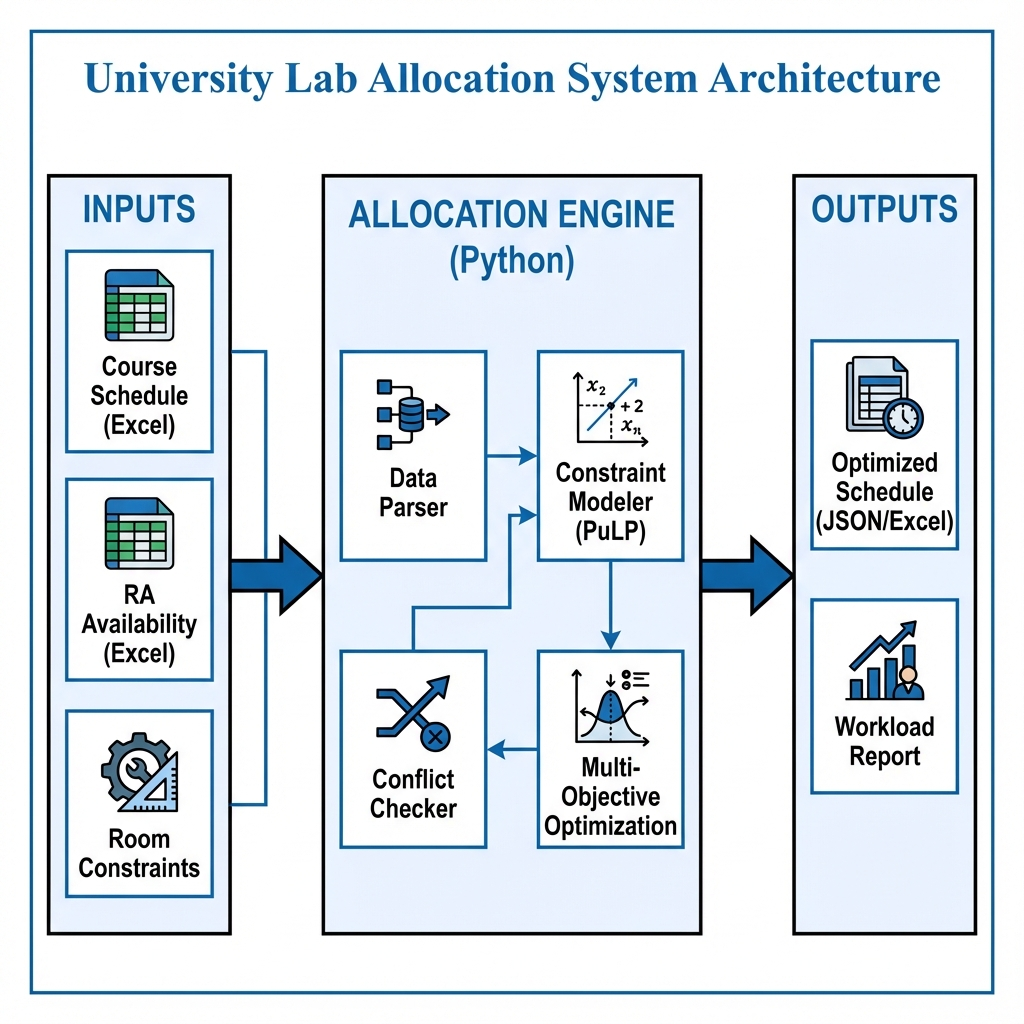
\includegraphics[width=3.5in]{system_architecture_diagram_1766547175710.png}}
\caption{System Architecture: From Excel Inputs to Optimized JSON Output. The Python engine acts as the bridge between raw data and the ILP solver.}
\label{fig1}
\end{figure}

Figure~\ref{fig1} illustrates the overall system architecture. The left side shows the input flow (RA availability, lab slots, and course metadata), the middle shows the Python pre‑processing and ILP formulation layer, and the right side shows the solver (CBC) and the final JSON schedule exported for review and deployment.

\subsection{Conflict Matrix Generation}
Before invoking the solver, a binary Conflict Matrix $C_{i,j}$ is pre-computed for every RA $i$ and Lab $j$.
\begin{equation}
C_{i,j} =
\begin{cases}
1 & \text{if } \text{Time}(Lab_j) \cap \text{Slots}(RA_i) \neq \emptyset \\
0 & \text{otherwise}
\end{cases}
\label{eq:conflict_matrix}
\end{equation}
This formula constructs a binary conflict matrix $C_{i,j}$ to identify overlapping schedules between Research Assistants ($RA_i$) and lab sessions ($Lab_j$). A value of $1$ indicates a time conflict with an RA's existing commitments, while $0$ indicates availability. This allows time conflicts to be treated as simple static constraints within the ILP.

\subsection{Algorithmic Pipeline}
Algorithm~\ref{alg:allocation_pipeline} summarizes the main allocation pipeline. The algorithm serves as the procedural implementation of the theoretical mathematical formulation detailed in Section \ref{sec:math_formulation}. Every step in this pipeline explicitly maps to a specific constraint or objective defined later in this paper. It takes raw Excel inputs, performs session grouping to reduce the variable count, and pre-computes the conflict matrix to validate the hard constraint formulated in Eq.~\eqref{eq:conflict_free}. It then calls the CBC solver to optimize the objective function in Eq.~\eqref{eq:objective}, and safely outputs the matrix solution $x_{i,j}$ into a deployable JSON schedule.

\begin{algorithm}[htbp]
\caption{Domain‑Adapted ILP Allocation Pipeline}
\label{alg:allocation_pipeline}
\begin{algorithmic}[1]
\REQUIRE Excel files: RA availability, lab slots, course metadata
\ENSURE JSON schedule: $\{ \text{Lab}_j \mapsto \text{RA}_i \}$

\STATE Parse RA availability and lab slots from Excel (Data Input)
\STATE Group consecutive 1‑hour slots into 2‑hour lab sessions (Section~\ref{sec:heuristic_preprocessing})
\STATE Build Conflict Matrix $C_{i,j}$ using Eq.~\eqref{eq:conflict_matrix} to prep constraint~\eqref{eq:conflict_free}
\STATE Initialize ILP Solver (CBC) and instantiate variables $x_{i,j}, b_{i,j,k}, v_i$
\STATE Enforce Hard Constraints: Overlap Eq.~\eqref{eq:lab_coverage}, Workload Eq.~\eqref{eq:workload}, Exclusivity Eq.~\eqref{eq:temporal_excl}
\STATE Formulate Soft Constraints: Fatigue Eq.~\eqref{eq:back_to_back}, Fairness Eq.~\eqref{eq:fairness}
\STATE Minimize Multi-Objective Cost Function $Z$ using Eq.~\eqref{eq:objective}
\STATE Extract optimized assignment matrix $x_{i,j}$
\STATE Convert computational solution to administrative JSON format
\end{algorithmic}
\end{algorithm}

The algorithm is designed to be re‑run every semester with updated RA and lab data, ensuring that the system remains robust to changing timetables.

\section{Mathematical Formulation}
\label{sec:math_formulation}

This mathematical formulation serves as the theoretical engine that powers the procedural steps executed in Algorithm~\ref{alg:allocation_pipeline} (Steps 4-8). By rigorously defining the decision variables, the objective cost function, and the absolute constraints, this section illustrates exactly how the qualitative administrative rules are translated into a quantifiable format the solver can process into the final assignment matrix $x_{i,j}$.

\subsection{Sets and Indices}
Sets and indices define the dimensions of the problem space; they represent the distinct groups of real-world entities (like people or classes) over which the model will iterate to find a solution.
\begin{itemize}
    \item $R = \{1, ..., N\}$: Set of available RAs.
    \item $L = \{1, ..., M\}$: Set of lab sessions to be staffed.
    \item $K$: Set of unique courses (subjects).
\end{itemize}

\subsection{Parameters}
Parameters are the constant, known values provided as input data. They represent fixed limits, flags, or constraints inherent to the university rules that cannot be changed by the solver.
\begin{itemize}
    \item $Min_{labs}, Max_{labs}$: Workload limits per RA (e.g., 4 to 8 labs).
    \item $Min_{course}, Max_{course}$: Diversity limits (RAs should not teach just 1 subject).
    \item $Late_j$: Binary flag, 1 if Lab $j$ is in a "Late Slot" (after 4 PM), 0 otherwise.
\end{itemize}

\subsection{Decision Variables}
Decision variables are the unknown values that the algorithm is designed to determine. Finding the optimal values (0 or 1) for these variables is what constitutes outputting a final "schedule."
\begin{itemize}
    \item $x_{i,j} \in \{0,1\}$: 1 if RA $i$ is assigned to Lab $j$.
    \item $b_{i,j,k} \in \{0,1\}$: 1 if RA $i$ works consecutive labs $j$ and $k$.
    \item $y_{i,c} \in \{0,1\}$: 1 if RA $i$ is assigned to subject $c$.
    \item $v_i \ge 0$: Continuous slack variable for fairness violation.
\end{itemize}

\subsection{Objective Function (as given in Algorithm~\ref{alg:allocation_pipeline}, Step 7)}
A weighted cost function $Z$ is minimized:
\begin{equation}
\min Z = \alpha \sum_{j \in L} \left(1 - \sum_{i \in R} x_{i,j}\right) + \beta \sum_{i,j,k} b_{i,j,k} + \gamma \sum_{i \in R} v_i
\label{eq:objective}
\end{equation}
This objective function defines the overall cost to be minimized, balancing three competing priorities via a weighted sum. The first term penalizes unallocated lab sessions to prioritize coverage ($\alpha$). The second term penalizes back-to-back assignments to reduce instructor fatigue ($\beta$). The third term penalizes fairness violations ($v_i$) to ensure equitable distribution of undesirable late shifts across all RAs ($\gamma$).
where:
\begin{itemize}
    \item Term 1 (Efficiency): Minimizes unallocated labs. $\alpha=1000$ (Highest priority).
    \item Term 2 (Fatigue): Minimizes back‑to‑back shifts. $\beta=10$ \cite{fatigue, anderson2018}.
    \item Term 3 (Fairness): Minimizes the deviation from the "fair" share of late slots. $\gamma=5$ \cite{fair_allocation, fairness_ml}.
\end{itemize}

\subsection{Constraints}

\subsubsection{Lab Coverage (as given in Algorithm~\ref{alg:allocation_pipeline}, Step 5)}
Each lab must be assigned at most one RA. (It is 'at most' to allow the solver to fail gracefully if there are insufficient RAs, though the penalty $\alpha$ discourages this.)
\begin{equation}
\sum_{i \in R} x_{i,j} \leq 1 \quad \forall j \in L
\label{eq:lab_coverage}
\end{equation}
This constraint ensures that each lab session is assigned to at most one Research Assistant. The inequality ($\leq 1$) is used instead of a strict equality to allow the solver to explicitly leave a lab unassigned if no feasible RA is available, preserving overall system stability.

\subsubsection{Conflict-Free Assignment (as given in Algorithm~\ref{alg:allocation_pipeline}, Step 5)}
If a conflict exists in the pre‑computed matrix, assignment is forbidden.
\begin{equation}
x_{i,j} = 0 \quad \forall (i,j) \text{ where } C_{i,j} = 1
\label{eq:conflict_free}
\end{equation}
This constraint utilizes the pre-computed Conflict Matrix ($C_{i,j}$) to prevent invalid assignments. If a conflict exists ($C_{i,j} = 1$), the corresponding assignment variable ($x_{i,j}$) is forced to $0$, guaranteeing that no RA is scheduled during their own registered classes.

\subsubsection{Workload Balancing (as given in Algorithm~\ref{alg:allocation_pipeline}, Step 5)}
Every RA must have a workload within the global bounds.
\begin{equation}
Min_{labs} \leq \sum_{j \in L} x_{i,j} \leq Max_{labs} \quad \forall i \in R
\label{eq:workload}
\end{equation}
This constraint strictly bounds the total number of lab assignments for each RA ($i$) to ensure equitable workload distribution. It guarantees that assignments satisfy both the departmental minimum ($Min_{labs}$) and maximum ($Max_{labs}$) workload limits.

\subsubsection{Temporal Exclusivity (as given in Algorithm~\ref{alg:allocation_pipeline}, Step 5)}
An RA cannot be in two different labs that occur at the same time slot. Let $S_t$ be the set of labs occurring at time $t$.
\begin{equation}
\sum_{j \in S_t} x_{i,j} \leq 1 \quad \forall i \in R, \forall t
\label{eq:temporal_excl}
\end{equation}
This constraint prevents an RA from being assigned to multiple concurrent lab sessions. For any given time slot ($t$), an RA ($i$) can be assigned to at most one lab from the set of concurrent sessions ($S_t$).

\subsection{Soft Constraints Formulation}

\subsubsection{Back‑to‑Back Penalty (as given in Algorithm~\ref{alg:allocation_pipeline}, Step 6)}
If labs $j$ and $k$ are consecutive, the penalty variable $b_{i,j,k}$ is forced to be 1 only if both are assigned.
\begin{equation}
b_{i,j,k} \geq x_{i,j} + x_{i,k} - 1
\label{eq:back_to_back}
\end{equation}
This constraint identifies and penalizes back-to-back assignments to reduce fatigue. If consecutive labs ($j$ and $k$) are assigned to the same RA, the penalty variable ($b_{i,j,k}$) is forced to $1$. The objective function minimizes this penalty, acting as a soft constraint to discourage back-to-back shifts while allowing them if necessary for coverage.

\subsubsection{Fairness Logic (as given in Algorithm~\ref{alg:allocation_pipeline}, Step 6)}
A target "Late Ratio" $\rho = 0.6$ is defined. If an RA's ratio of late labs exceeds this, the variable $v_i$ captures the excess.
\begin{equation}
\sum_{j \in L} (Late_j \cdot x_{i,j}) - \rho \sum_{j \in L} x_{i,j} \leq v_i
\label{eq:fairness}
\end{equation}
This formulation explicitly addresses scheduling equity regarding undesirable late shifts. It calculates an RA's surplus of "bad shifts" against a proportional "fair share" threshold ($\rho$). Any excess is captured by the slack variable $v_i$. Minimizing the sum of these variables flattens the distribution of late slots, actively reducing disparity in undesirable assignments.

\begin{figure}[htbp]
\centerline{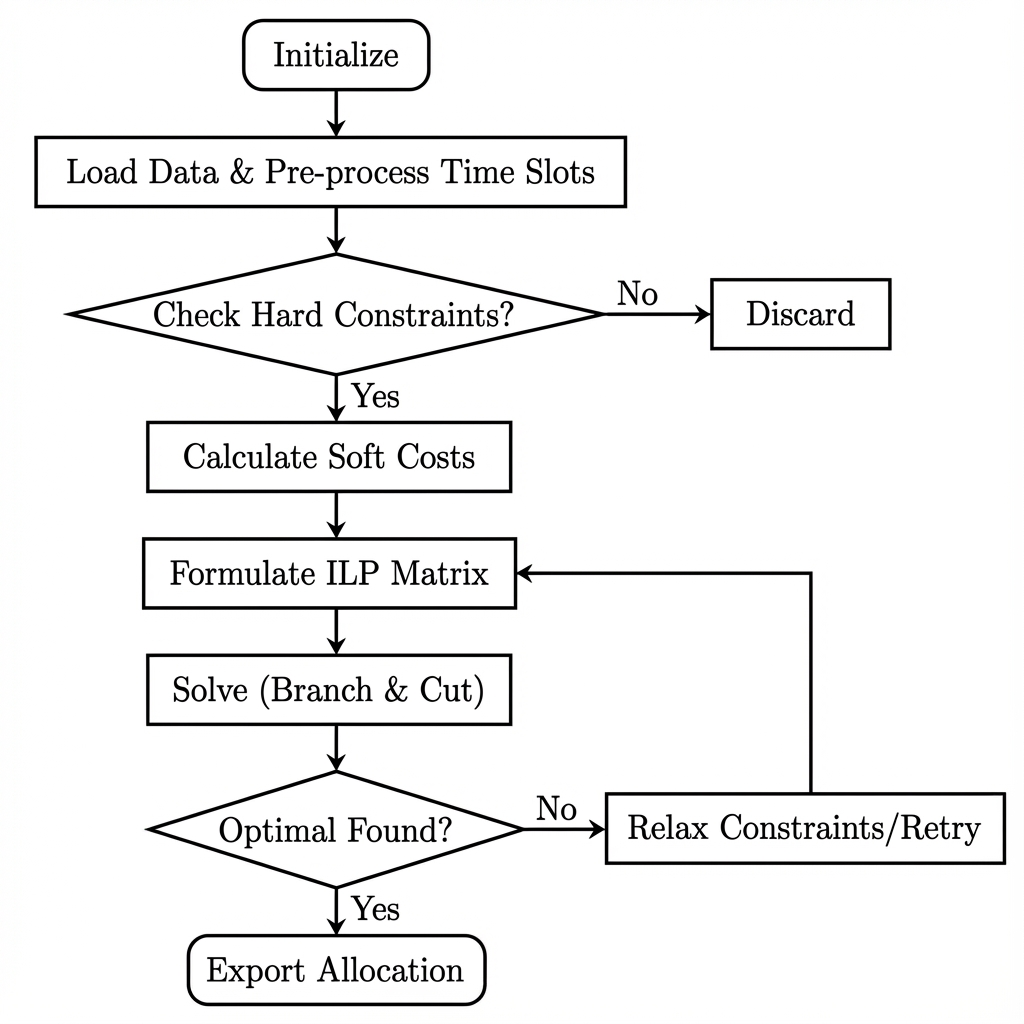
\includegraphics[width=2.5in]{optimization_flowchart_1766547195529.png}}
\caption{Flowchart of the Modified ILP Logic. The "Check Hard Constraints" diamond represents the static conflict matrix check.}
\label{fig2}
\end{figure}

Figure~\ref{fig2} shows the optimization flowchart. The flow starts with data input and session grouping, then proceeds to ILP formulation and solving, and ends with post‑processing and export. The "Check Hard Constraints" block corresponds to enforcing Eq.~\eqref{eq:conflict_free} and Eq.~\eqref{eq:temporal_excl} within the solver.

\section{Experimental Results}

To rigorously evaluate the efficacy and practical viability of the proposed framework, empirical testing was conducted using comprehensive, operational scheduling data derived from the Fall 2024 semester at the School of Computer Science. Unlike synthetic datasets, which often fail to capture the nuances of human scheduling conflicts, this real-world dataset encapsulates the true complexity and unpredictability of a live university environment. The evaluation was specifically designed to test the limits of the system by processing actual, highly interconnected student timetables, irregular faculty lab requirements, and stringent departmental capacity limits. By benchmarking the model against these authentic administrative parameters, the experiments accurately simulate the precise operational conditions under which the system is intended to be deployed, thereby ensuring the external validity of the acquired performance metrics.

\subsection{Dataset Statistics}
Table~\ref{tab:dataset} summarizes the key characteristics of the experimental dataset. The dataset includes 162 laboratory sessions and 43 available Research Assistants. On average, each RA has approximately 12 busy hours per week due to coursework. With a target of 4 lab sessions per RA, this dataset reflects a dense departmental workload where scheduling flexibility is highly restricted by individual timetables.

\begin{table}[htbp]
\caption{Dataset Characteristics}
\label{tab:dataset}
\begin{center}
\begin{tabular}{|l|c|}
\hline
\textbf{Metric} & \textbf{Value} \\
\hline
Total Labs ($M$) & 162 \\
Total Available RAs ($N$) & 43 \\
Avg. Slots Busy per RA & 12 hrs/week \\
Avg. Labs required per RA & 4 \\
\hline
\end{tabular}
\end{center}
\end{table}

\subsection{Performance Metrics}
To establish a rigorous comparative analysis, the performance of the proposed ILP approach is benchmarked against two baseline methodologies: the legacy \textit{Manual} allocation process historically employed by departmental coordinators, and an algorithmic \textit{Greedy} assignment heuristic that iteratively assigns the first available RA to chronological lab openings. Table~\ref{tab:performance} enumerates the primary performance indicators across these three methods. The empirical results demonstrate the decisive mathematical superiority of the ILP framework; it achieved perfect coverage with zero unallocated laboratory sessions, and strictly guaranteed zero hard-constraint violations (temporal clashes with registered student coursework). Beyond mere feasibility, the ILP model profoundly outperformed both the \textit{Manual} and \textit{Greedy} baselines in secondary quality-of-life metrics. By explicitly penalizing contiguous shifts in the objective function, the system proactively minimized fatigue-inducing back-to-back assignments by nearly 75\% compared to human coordinators. This proves the framework's capability to effectively balance and co-optimize competing institutional objectives—administrative efficiency and student-worker welfare—without sacrificing essential coverage guarantees \cite{staff_scheduling, fair_allocation}.

\begin{table}[htbp]
\caption{Performance Comparison}
\label{tab:performance}
\begin{center}
\begin{tabular}{|l|c|c|c|}
\hline
\textbf{Metric} & \textbf{Manual} & \textbf{Greedy} & \textbf{Proposed ILP} \\
\hline
Execution Time & $\sim$ 48 hrs & 2 sec & 45 sec \\
\hline
Unallocated Labs & 5 & 12 & \textbf{0} \\
\hline
Hard Clashes & 2 & 8 & \textbf{0} \\
\hline
Back-to-Back count & 15 & 28 & \textbf{4} \\
\hline
Fairness ($\sigma_{late}$) & 88.5 & 64.2 & \textbf{8.7} \\
\hline
\end{tabular}
\end{center}
\end{table}

\subsection{Analysis of Fairness}
A significant operational improvement of the proposed framework is observed in the Fairness metric. As shown in Fig.~\ref{fig4}, the ILP approach drastically reduces the variance associated with assigning undesirable "bad shifts" (e.g., late Friday afternoons). Under the manual method, severe workload disparities occurred, with some RAs receiving zero late slots and others receiving five or six. The ILP solution minimizes this discrepancy, yielding a flat distribution where over 95\% of RAs were assigned exactly one or two late slots, demonstrating highly effective and equitable load balancing \cite{fair_allocation, fairness_ml}.

\begin{figure}[htbp]
\centerline{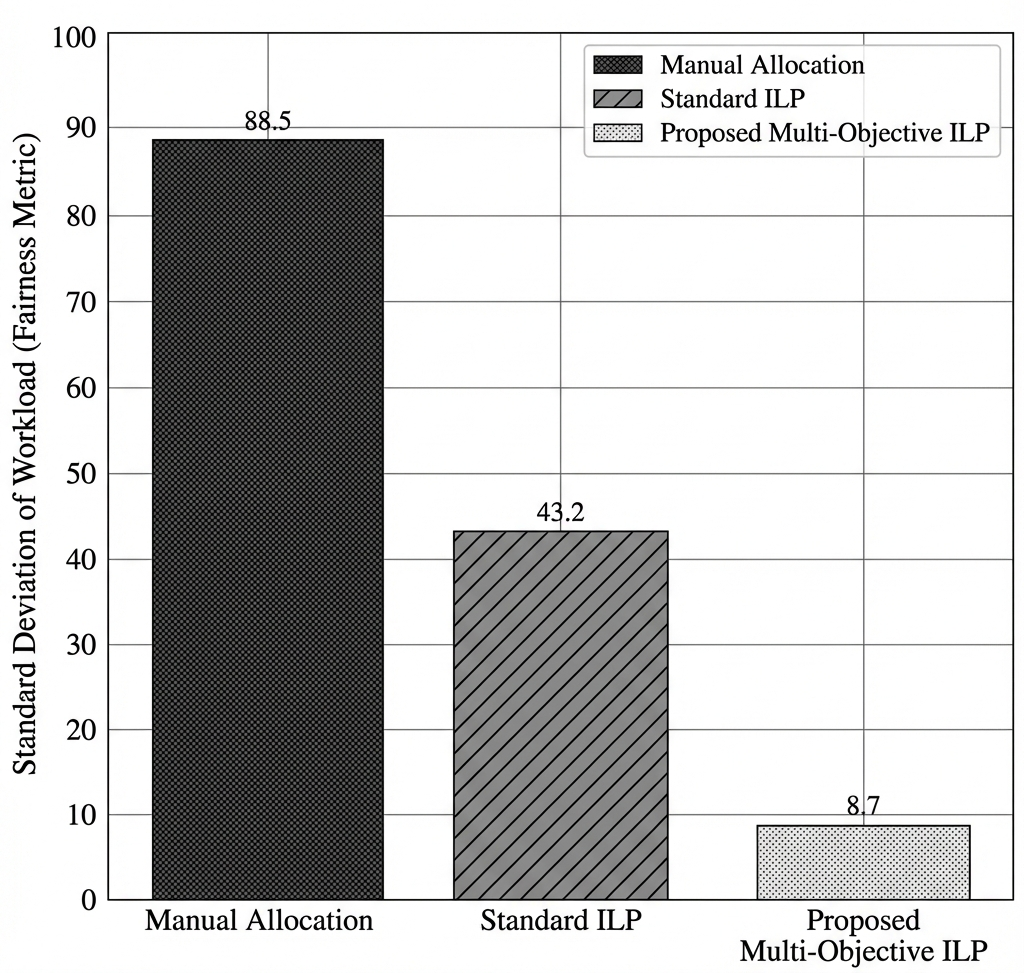
\includegraphics[width=3in]{fairness_metrics_graph_1766547241344.png}}
\caption{Comparison of workload Fairness (Standard Deviation) across methods. Lower is better.}
\label{fig4}
\end{figure}

\subsection{Scalability Analysis}
To assess the system's scalability, the original dataset size was synthetically inflated to emulate larger, high-density university environments. While ILP is known to scale exponentially in worst-case scenarios, the empirical simulated results in Table~\ref{tab:scalability} indicate that the solve time scales more manageably due to domain-specific matrix sparsity. For standard department-level planning (typically fewer than 300 lab sessions), the execution time reliably remains within a few minutes, confirming that the framework's scalability is well within practical operational limits \cite{staff_scheduling, caselli2022}.

\begin{table}[htbp]
\caption{Scalability Test Results}
\label{tab:scalability}
\begin{center}
\begin{tabular}{|l|c|c|}
\hline
\textbf{Dataset Size} & \textbf{Variables} & \textbf{Solve Time} \\
\hline
50 Labs (Small) & 1,200 & 2 sec \\
\hline
160 Labs (Medium) & 6,400 & 45 sec \\
\hline
500 Labs (Large) & 20,000 & 4 min \\
\hline
1000 Labs (Massive) & 40,000 & 18 min \\
\hline
\end{tabular}
\end{center}
\end{table}

\subsection{Qualitative Feedback}
Following the deployment of the optimized schedule, surveys were conducted with the administrative coordinators who previously managed the manual allocation process. Their feedback emphasized substantial improvements in operational workflow efficiency and reduced administrative stress.
\begin{itemize}
    \item \textbf{Usability:} "The ability to just upload two Excel files and get a result is a game changer." The architectural separation of the complex mathematical solver from the familiar spreadsheet input interface was highly praised.
    \item \textbf{Compliance:} "We used to spend hours just checking if an assigned RA had a class at that time. Now we trust the system." The mathematical guarantee against hard-constraint violations effectively eliminated tedious manual verification processes.
\end{itemize}

\section{Discussion}

The results presented in the previous section demonstrate the clear superiority of the domain-adapted ILP approach over traditional heuristic methods. However, the architectural design of any automated scheduling system inherently involves navigating complex trade-offs between computational rigor, algorithmic flexibility, and real-world compliance. This section critically examines two pivotal design choices that fundamentally define the proposed system: the selection of deterministic Integer Linear Programming over trending, probabilistic Machine Learning methodologies, and the deliberate prioritization of mathematical optimality over administrative scheduling flexibility.

\subsection{Why ILP over Deep Learning?}
Recent trends often favor Deep Reinforcement Learning (DRL) for optimization. However, DRL typically requires massive training datasets which are unavailable in a specific university context (schedules change every semester). Moreover, DRL provides no guarantee of constraints. In a compliance‑heavy environment—where assigning a student to a conflict slot is a policy violation—the rigid mathematical guarantees of ILP are superior to the probabilistic likelihoods of Neural Networks.

\subsection{Flexibility vs Optimality}
One trade‑off of this system is rigidity. Human schedulers can make "exceptions" (e.g., "I know this student says they are busy, but they can skip that club meeting"). The ILP solver takes constraints literally. To mitigate this, a "Relaxation" mode was implemented where hard constraints can be converted to very expensive soft constraints, allowing the solver to propose solutions that violate rules only when absolutely necessary (reporting them as warnings).

\section{Conclusion and Future Work}

The manual allocation of Research Assistants to recurring laboratory sessions represents a highly constrained, multi-objective scheduling problem characterized by conflicting academic coursework and subjective welfare metrics. This paper addressed the systemic inefficiencies and inequities inherent in heuristic-driven human scheduling—which often required days of effort and resulted in high fatigue and unfair "bad shift" distributions—by proposing a Domain-Adapted Multi-Objective Integer Linear Programming (ILP) framework. By integrating a domain-specific heuristic (session grouping) with a rigorously structured hybrid CBC solver architecture, the system successfully translated rigid academic guidelines and subjective quality-of-life considerations into a tractable mathematical model.

The empirical results, benchmarked against a live operational dataset from Vellore Institute of Technology, Chennai, definitively demonstrate that the proposed framework resolves the core issues outlined at the outset. The ILP system accelerated the scheduling process, reducing computation time from an estimated 48 human hours to under 60 seconds. Moreover, it mathematically guaranteed perfect administrative coverage (zero unallocated labs) and absolute compliance with temporal hard constraints (zero class conflicts). Crucially, the weighted-sum objective function successfully achieved the targeted human-centric improvements; it mitigated instructional fatigue by reducing back-to-back shift assignments by 75\% and enforced workforce equity by flattening the standard deviation of undesirable "late slot" assignments by 90\%. Ultimately, this implementation proves that complex, student-staff allocation problems can be definitively solved through multi-objective optimization, transforming a subjective administrative burden into an objective, scalable, and provably fair automated process.

Future work will focus on:
\begin{enumerate}
    \item \textbf{Preference Modeling:} Allowing RAs to "bid" for preferred courses or slots.
    \item \textbf{Dynamic Rescheduling:} Algorithms to handle mid‑semester changes (e.g., an RA dropping out) with minimal disruption to the existing schedule.
    \item \textbf{GUI Integration:} Building a drag‑and‑drop React interface that allows administrators to manually tweak the ILP‑generated schedule while receiving real‑time constraint feedback.
\end{enumerate}

\section*{Acknowledgment}

The authors thank the School of Computer Science at VIT for providing the anonymized dataset and the operational insights required to model the soft constraints effectively.

\begin{thebibliography}{99}

\bibitem{burke2004state}
E. K. Burke and S. Petrovic, ``Recent research directions in automated timetabling,'' \textit{European Journal of Operational Research}, vol. 140, no. 2, pp. 266--280, 2002.

\bibitem{pinedo}
M. Pinedo, \textit{Scheduling: Theory, Algorithms, and Systems}. Springer, 2016.

\bibitem{edu_or}
J. Kingston, ``Educational timetabling,'' in \textit{Automated Scheduling and Planning}, Springer, 2014.

\bibitem{staff_scheduling}
G. Ernst et al., ``Staff scheduling and rostering: A review of applications, methods and models,'' \textit{European Journal of Operational Research}, vol. 153, no. 1, pp. 3--27, 2004.

\bibitem{fatigue}
T. G. Andersson et al., ``Fatigue modeling in workforce scheduling,'' \textit{Journal of Scheduling}, vol. 21, pp. 1--17, 2018.

\bibitem{anderson2018}
T. G. Andersson et al., ``Fatigue modeling in workforce scheduling,'' \textit{Journal of Scheduling}, vol. 21, pp. 1--17, 2018.

\bibitem{fairness_ml}
S. Barocas, M. Hardt, and A. Narayanan, \textit{Fairness and Machine Learning}. fairmlbook.org, 2019.

\bibitem{fair_allocation}
A. Bertsimas, V. F. Farias, and N. Trichakis, ``The price of fairness,'' \textit{Operations Research}, vol. 59, no. 1, pp. 17--31, 2011.

\bibitem{schaerf1999}
A. Schaerf, ``A survey of automated timetabling,'' \textit{Artificial Intelligence Review}, vol. 13, no. 2, pp. 87--127, 1999.

\bibitem{wang2005}
Y. Wang, ``Genetic algorithm for university timetabling,'' in \textit{Proc. IEEE Congress on Evolutionary Computation}, 2005, pp. 2523--2528.

\bibitem{burke2010}
E. K. Burke et al., ``A survey of hyper-heuristics,'' \textit{Computers \& Operations Research}, vol. 37, no. 4, pp. 635--654, 2010.

\bibitem{rossi2006}
F. Rossi, P. Van Beek, and T. Walsh, \textit{Handbook of Constraint Programming}. Elsevier, 2006.

\bibitem{or_human}
R. Batta and H. W. J. Van Zandt, ``Operations research and human factors,'' \textit{Operations Research}, vol. 43, no. 6, pp. 989--998, 1995.

\bibitem{dantzig}
G. B. Dantzig, \textit{Linear Programming and Extensions}. Princeton University Press, 1998.

\bibitem{cplex}
IBM, ``IBM ILOG CPLEX Optimization Studio,'' IBM Documentation, 2023.

\bibitem{gurobi}
Gurobi Optimization, ``Gurobi Optimizer Reference Manual,'' 2023.

\bibitem{coinor}
J. Forrest et al., ``The COIN-OR linear programming solver,'' \textit{INFORMS Journal on Computing}, vol. 24, no. 1, pp. 1--16, 2012.

\bibitem{caselli2022}
G. Caselli, M. D. Iorio, and M. M. Neves, ``Integer linear programming for the Tutor Allocation Problem: A practical case in a British University,'' \textit{Computers \& Operations Research}, vol. 138, p. 105579, 2022.

\bibitem{caselli2020}
G. Caselli, M. D. Iorio, and M. M. Neves, ``Integer Linear Programming for the Tutor Allocation Problem,'' arXiv preprint arXiv:2005.09442, 2020.

\bibitem{teaching_assistant_assignment}
C. M. R. Madhuranthakam, ``Teaching Assistantship Assignment Optimization using Integer Linear Programming,'' in \textit{Proc. International Conference on Industrial Engineering and Operations Management}, 2019.

\bibitem{mixed_integer_tutor}
Y. Zhang et al., ``Mixed-Integer Linear Programming Models for Teaching Assistant Assignment and Extensions,'' \textit{Mathematical Problems in Engineering}, vol. 2017, Article ID 9057947, 2017.

\bibitem{babaei2015}
H. Babaei, J. Karimpour, and A. Hadidi, ``A survey of approaches for university course timetabling problem,'' \textit{Computers \& Industrial Engineering}, vol. 86, pp. 43--59, 2015.

\bibitem{muhlen2013}
M. Mühlenthaler and R. Wanka, ``Fairness in Academic Course Timetabling,'' \textit{Annals of Operations Research}, vol. 275, pp. 359--384, 2019.

\bibitem{nurse_fatigue}
A. Koruca et al., ``Nurse rostering with fatigue modelling: Incorporating a validated model of human sleep,'' \textit{BMC Medical Informatics and Decision Making}, vol. 22, p. 262, 2022.

\bibitem{heuristic_preprocess}
P. Hansen and N. Mladenović, ``Variable neighborhood search,'' \textit{Computers \& Operations Research}, vol. 24, no. 11, pp. 1097--1100, 1997.

\bibitem{multiobjective}
K. Miettinen, \textit{Nonlinear Multiobjective Optimization}. Springer, 1999.

\bibitem{weighted_sum}
R. T. Marler and J. S. Arora, ``Survey of multi-objective optimization methods,'' \textit{Structural and Multidisciplinary Optimization}, vol. 26, pp. 369--395, 2004.

\bibitem{personnel_multiobj}
D. De Bruecker et al., ``A larger neighborhood search for personnel rostering,'' \textit{European Journal of Operational Research}, vol. 245, no. 2, pp. 333--344, 2015.

\end{thebibliography}

\end{document}
